% Copyright (C) 2012 Raniere Silva
%
% This work is licensed under the Creative Commons
% Attribution-ShareAlike 3.0 Unported License. To view a copy of this
% license, visit <http://creativecommons.org/licenses/by-sa/3.0/>.
%
% This work is distributed in the hope that it will be useful, but
% WITHOUT ANY WARRANTY; without even the implied warranty of
% MERCHANTABILITY or FITNESS FOR A PARTICULAR PURPOSE.

\documentclass[]{beamer}

\usetheme{CambridgeUS}
\let\Tiny=\tiny % Redefine at least \Tiny for avoid warning

\usepackage[utf8]{inputenc}
\usepackage[T1]{fontenc}

\usepackage[brazil]{babel}
\usepackage{indentfirst}
\uselanguage{brazil}
\languagepath{brazil}
\deftranslation[to=brazil]{Example}{Exemplo}

\usepackage{url}
\usepackage{hyperref}
\usepackage{breakurl}

\usepackage{xmpincl}

\usepackage{amsmath}
\usepackage{amsfonts}
\usepackage{amssymb}
\usepackage{amsthm}
\usepackage{breqn}

\usepackage{multicol}
\usepackage{multirow}
\usepackage{array}

\usepackage{graphicx}
\usepackage{subfigure}
\usepackage{wrapfig}
\usepackage{tikz}

\usepackage{algorithmic}
\algsetup{linenosize=\small}

\usepackage{algorithm}
\floatname{algorithm}{Algoritmo}

\usepackage{textcomp}
\usepackage{listings}
\lstset{
% language=Octave,
basicstyle=\ttfamily\scriptsize,
columns=flexible,
% numbers=left,
% numberstyle=\footnotesize,
% stepnumber=5,
% numbersep=5pt,
% backgroundcolor=\color{white},
% showspaces=false,
% showstringspaces=false,
% showtabs=false,
% frame=single,
tabsize=4,
captionpos=t,
breaklines=true,
breakatwhitespace=false,
% caption={\texttt{\lstname}},
% escapeinside={\%*}{*)},
% morekeywords={#},
upquote=true,
}

% Index
\usepackage{makeidx}
\makeindex


\newcommand{\flang}[1]{\textit{#1}}

\hypersetup{
pdftitle={EPUB e o Futuro da Publicação},
pdfauthor={Raniere Silva},
pdfsubject={EPUB3, ebook, livro digita, livro eletrônico, padrões abertos},
pdfcreator={Raniere Silva},
pdfkeywords={EPUB3, ebook, livro digita, livro eletrônico, padrões abertos}
}
\includexmp{epub_itf}

\newtheorem{defi}{Definição}
\newtheorem{prop}{Proposição}

\renewcommand{\algorithmicrequire}{\textbf{Entrada:}}
\renewcommand{\algorithmicensure}{\textbf{Saída:}}
\renewcommand{\algorithmicend}{\textbf{fim}}
\renewcommand{\algorithmicif}{\textbf{se}}
\renewcommand{\algorithmicthen}{\textbf{ent\~{a}o}}
\renewcommand{\algorithmicelse}{\textbf{caso contr\'{a}rio}}
\renewcommand{\algorithmicendif}{\algorithmicend}
\renewcommand{\algorithmicfor}{\textbf{para}}
\renewcommand{\algorithmicforall}{\textbf{para todo}}
\renewcommand{\algorithmicdo}{\textbf{fa\c{c}a}}
\renewcommand{\algorithmicendfor}{\algorithmicend}
\renewcommand{\algorithmicwhile}{\textbf{enquanto}}
\renewcommand{\algorithmicendwhile}{\algorithmicend}
\renewcommand{\algorithmicrepeat}{\textbf{repita}}
\renewcommand{\algorithmicuntil}{\textbf{at\'{e}}}
\renewcommand{\algorithmicreturn}{\textbf{retorne}}
\renewcommand{\algorithmiccomment}[1]{\hspace{2em}/* #1 */}

\renewcommand{\lstlistingname}{C\'{o}digo}

\begin{document}
\title[epub]{epub e o futuro da publica\c{c}\~{a}o}
\author[Raniere Silva]{Raniere Gaia Costa da
Silva\footnote{ra092767@ime.unicamp.br}}
\date{13/10/2012}

\begin{frame}
    \titlepage
\end{frame}

\begin{frame}
  \begin{block}{}
    Os arquivos desta apresentação encontram-se disponíveis \\
    em \url{https://github.com/r-gaia-cs/presentations}. \\
    \vspace{-33pt}
    \begin{flushright}
      \includegraphics[height=2cm]{../figures/forkme_right_red.png}
    \end{flushright}
  \end{block}

  \begin{block}{Licença}
    Salvo indicado o contrário, esta apresentação está licenciada sob a
    Licença Creative Commons Atribuição-CompartilhaIgual 3.0 Não Adaptada .
    Para ver uma cópia desta licença, visite
    \url{http://creativecommons.org/licenses/by/3.0/deep.pt_BR}.
    \begin{center}
      
\includegraphics{../figures/cc-by-sa.png}
    \end{center}
  \end{block}
\end{frame}

\begin{frame}
    \frametitle{~17000 a.C.}
    \begin{center}
        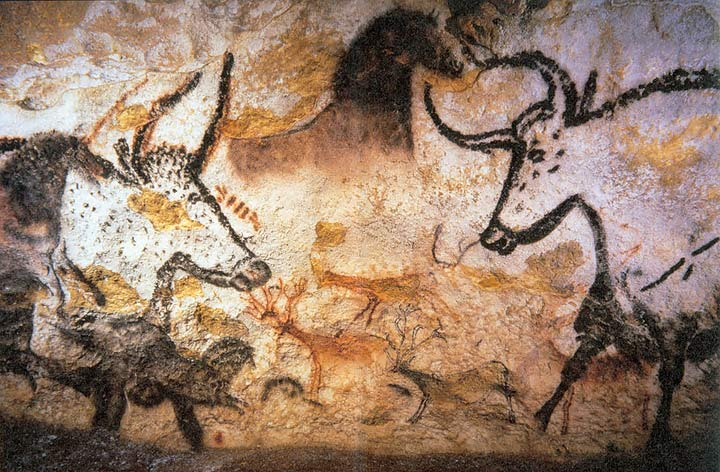
\includegraphics[height=0.6\textheight]{pictures/lascaux_painting.jpg}
    \end{center}

    \begin{tiny}
        A imagem acima, de Prof saxx, encontra-se dispon\'{i}vel em \url{http://pt.wikipedia.org/wiki/Ficheiro:Lascaux_painting.jpg} e regulada nos termos da licen\c{c}a Creative Commons - Atribui\c{c}\~{a}o - Partilha nos Mesmos Termos 3.0 N\~{a}o Adaptada.
    \end{tiny}
\end{frame}

\begin{frame}[t]
    \begin{center}
        \begin{tabular}{|c|c|c|c|c|}
            \hline
            Ano & \multicolumn{2}{|c|}{Produ\c{c}\~{a}o} & \multicolumn{2}{|c|}{Reprodu\c{c}\~{a}o} \\ \cline{2-5}
            & Custo & Tempo & Custo & Tempo \\ \hline
            ~17000 a.c. & +++++ & +++++ & +++++ & +++++  \\ \hline
        \end{tabular}
    \end{center}
\end{frame}

\begin{frame}
    \frametitle{~3000 a.C.}
    \begin{center}
        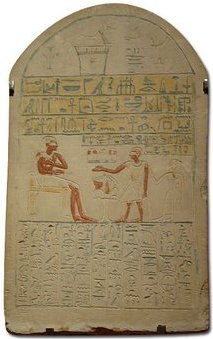
\includegraphics[height=0.6\textheight]{pictures/egyptian_funerary_stela.jpg}
    \end{center}

    \begin{tiny}
        A imagem acima, de Jeeny, encontra-se dispon\'{i}vel em \url{http://pt.wikipedia.org/wiki/Ficheiro:Egyptian_funerary_stela.jpg} e regulada nos termos da licen\c{c}a Creative Commons - Atribui\c{c}\~{a}o - Partilha nos Mesmos Termos 3.0 N\~{a}o Adaptada.
    \end{tiny}
\end{frame}

\begin{frame}[t]
    \begin{center}
        \begin{tabular}{|c|c|c|c|c|}
            \hline
            Ano & \multicolumn{2}{|c|}{Produ\c{c}\~{a}o} & \multicolumn{2}{|c|}{Reprodu\c{c}\~{a}o} \\ \cline{2-5}
            & Custo & Tempo & Custo & Tempo \\ \hline
            ~17000 a.C. & +++++ & +++++ & +++++ & +++++  \\ \hline
            ~3000 a.C & +++++ & +++++ & +++++ & +++++ \\ \hline
        \end{tabular}
    \end{center}
\end{frame}

\begin{frame}
    \frametitle{~1407 d.C.}
    \begin{center}
        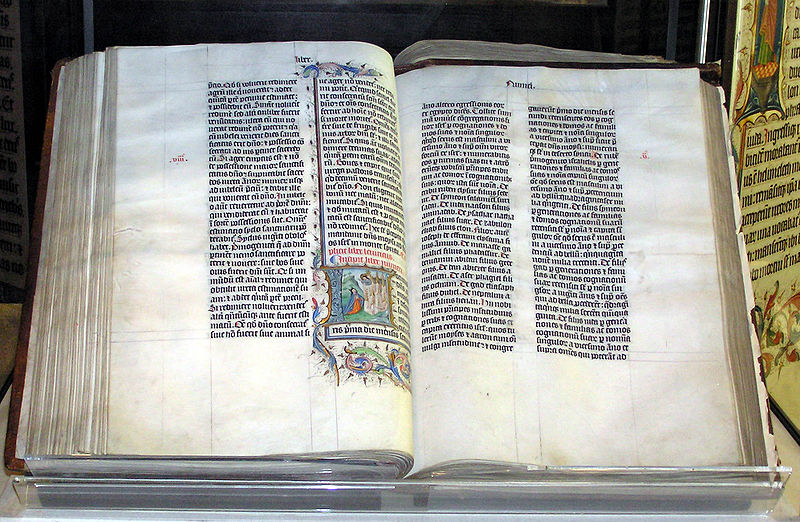
\includegraphics[height=0.6\textheight]{pictures/bible_malmesbury_arp.jpg}
    \end{center}

    \begin{tiny}
        A imagem acima, de Arpingstone, encontra-se dispon\'{i}vel em \url{http://pt.wikipedia.org/wiki/Ficheiro:Bible.malmesbury.arp.jpg} e regulada nos termos da licen\c{c}a Creative Commons - Atribui\c{c}\~{a}o - Partilha nos Mesmos Termos 3.0 N\~{a}o Adaptada.
    \end{tiny}
\end{frame}

\begin{frame}[t]
    \begin{center}
        \begin{tabular}{|c|c|c|c|c|}
            \hline
            Ano & \multicolumn{2}{|c|}{Produ\c{c}\~{a}o} & \multicolumn{2}{|c|}{Reprodu\c{c}\~{a}o} \\ \cline{2-5}
            & Custo & Tempo & Custo & Tempo \\ \hline
            ~17000 a.C. & +++++ & +++++ & +++++ & +++++  \\ \hline
            ~3000 a.C & +++++ & +++++ & +++++ & +++++ \\ \hline
            ~1407 d.C & ++++ & ++++ & ++++ & +++ \\ \hline
        \end{tabular}
    \end{center}
\end{frame}

\begin{frame}
    \frametitle{~1450 d.C.}
    \begin{center}
        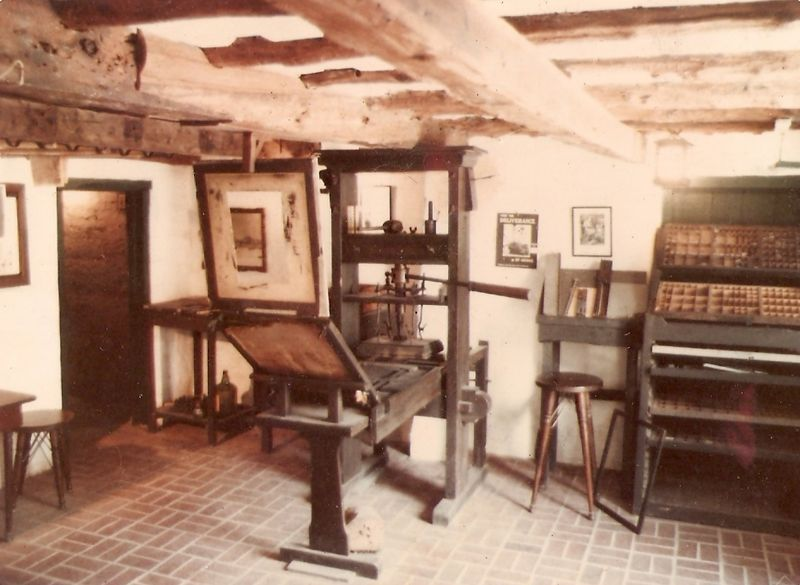
\includegraphics[height=0.6\textheight]{pictures/featherbed_alley_printshop_bermuda.jpg}
    \end{center}

    \begin{tiny}
        A imagem acima, de Aodhdubh, encontra-se dispon\'{i}vel em \url{http://en.wikipedia.org/wiki/File:Featherbed_Alley_Printshop_Bermuda.jpg} e regulada nos termos da licen\c{c}a Creative Commons - Atribui\c{c}\~{a}o - Partilha nos Mesmos Termos 3.0 N\~{a}o Adaptada.
    \end{tiny}
\end{frame}

\begin{frame}[t]
    \begin{center}
        \begin{tabular}{|c|c|c|c|c|}
            \hline
            Ano & \multicolumn{2}{|c|}{Produ\c{c}\~{a}o} & \multicolumn{2}{|c|}{Reprodu\c{c}\~{a}o} \\ \cline{2-5}
            & Custo & Tempo & Custo & Tempo \\ \hline
            ~17000 a.C. & +++++ & +++++ & +++++ & +++++  \\ \hline
            ~3000 a.C & +++++ & +++++ & +++++ & +++++ \\ \hline
            ~1407 d.C & ++++ & ++++ & ++++ & +++ \\ \hline
            ~1450 d.C & ++++ & ++++ & ++ & ++ \\ \hline
        \end{tabular}
    \end{center}
\end{frame}

\begin{frame}
    \frametitle{1978-\ldots}
    \begin{description}
        \item[1978] Donald Knuth lan\c{c}a TeX.
        \item[1979] David Fuchs lan\c{c}a DVI (device independent file format).
        \item[1982] John Warnock e Charles Geschke lan\c{c}a PostScript.
        \item[1985] Leslie Lamport lan\c{c}a LaTeX.
        \item[1991] John Warnock lan\c{c}a PDF (Portable Document Format).
    \end{description}
\end{frame}

\begin{frame}[fragile]
    \frametitle{LaTeX}
    \lstinputlisting{examples/latex_minimal.tex}
\end{frame}

\begin{frame}[fragile]
    \frametitle{LaTeX e matem\'{a}tica}
    \lstinputlisting{examples/latex_math.tex}
\end{frame}

\begin{frame}[fragile]
    \frametitle{LaTeX e c\'{o}digos}
    \lstinputlisting{examples/latex_codes.tex}
\end{frame}

\begin{frame}[t]
    \begin{center}
        \begin{tabular}{|c|c|c|c|c|}
            \hline
            & \multicolumn{2}{|c|}{Produ\c{c}\~{a}o} & \multicolumn{2}{|c|}{Reprodu\c{c}\~{a}o} \\ \cline{2-5}
            & Custo & Tempo & Custo & Tempo \\ \hline
            ~17000 a.C. & +++++ & +++++ & +++++ & +++++  \\ \hline
            ~3000 a.C & +++++ & +++++ & +++++ & +++++ \\ \hline
            ~1407 d.C & ++++ & ++++ & ++++ & +++ \\ \hline
            ~1450 d.C & ++++ & ++++ & ++ & ++ \\ \hline
            LaTeX  & + & ++ & + & + \\ \hline
        \end{tabular}
    \end{center}
\end{frame}

\begin{frame}
    \frametitle{1989-\ldots}
    \begin{description}
        \item[1989] Berners-Lee prop\~{o}e \textit{Internet-based hypertext system}.
        \item[1991] Publicado especifica\c{c}\~{o}es do HTML.
        \item[1995] Publicado especifica\c{c}\~{o}es do HTML 2.0.
        \item[1996] Criado World Wide Web Consortium (W3C) para manter as especifica\c{c}\~{o}es do HTML.
        \item[2008] Publicado ``esbo\c{c}o'' do HTML 5.0.
    \end{description}
\end{frame}

\begin{frame}[fragile]
    \frametitle{HTML}
    \lstinputlisting{examples/html_minimal.html}
\end{frame}

\begin{frame}[t]
    \begin{center}
        \begin{tabular}{|c|c|c|c|c|}
            \hline
            & \multicolumn{2}{|c|}{Produ\c{c}\~{a}o} & \multicolumn{2}{|c|}{Reprodu\c{c}\~{a}o} \\ \cline{2-5}
            & Custo & Tempo & Custo & Tempo \\ \hline
            ~17000 a.C. & +++++ & +++++ & +++++ & +++++  \\ \hline
            ~3000 a.C & +++++ & +++++ & +++++ & +++++ \\ \hline
            ~1407 d.C & ++++ & ++++ & ++++ & +++ \\ \hline
            ~1450 d.C & ++++ & +++ & ++ & ++ \\ \hline
            LaTeX  & + & ++ & + & + \\ \hline
            HTML & + & ++ & + & + \\ \hline
        \end{tabular}
    \end{center}
    \pause
    Nota: O LaTeX \'{e} est\'{a}tico enquanto que o HTML \'{e} din\^{a}mico.
\end{frame}

\begin{frame}[fragile]
    \frametitle{2004-\ldots}
    \begin{description}
        \item[2004] Sony lan\c{c}a Libri\'{e} EBR-1000EP no Jap\~{a}o, o primeiro \textit{e-book reader} com \textit{electronic paper display}.
        \item[2006] Sony lan\c{c}a PRS-500 Sony Reader nos Estados Unidos.
        \item[2007] Amazon lan\c{c}a Amazon Kindle.
    \end{description}

    \begin{tiny}
        \begin{center}
            \begin{tabular}{p{0.3\textwidth}p{0.3\textwidth}p{0.3\textwidth}}
                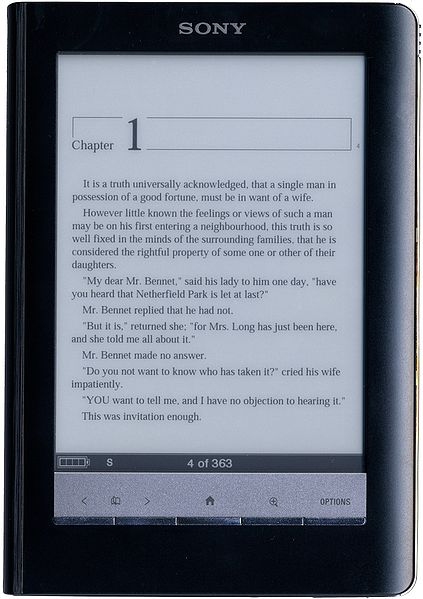
\includegraphics[height=0.25\textheight]{pictures/sony_reader.jpg} & 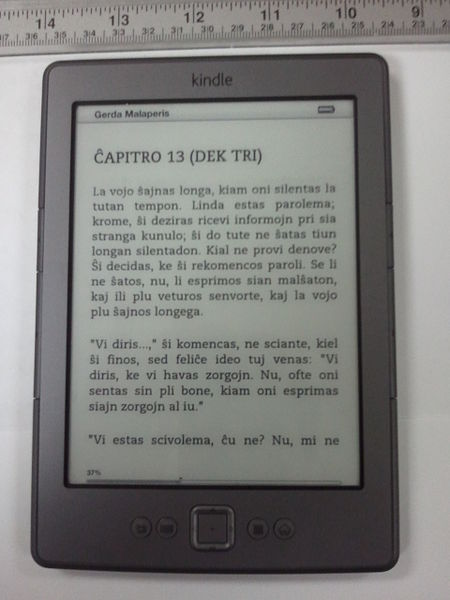
\includegraphics[height=0.25\textheight]{pictures/kindle4.jpg} &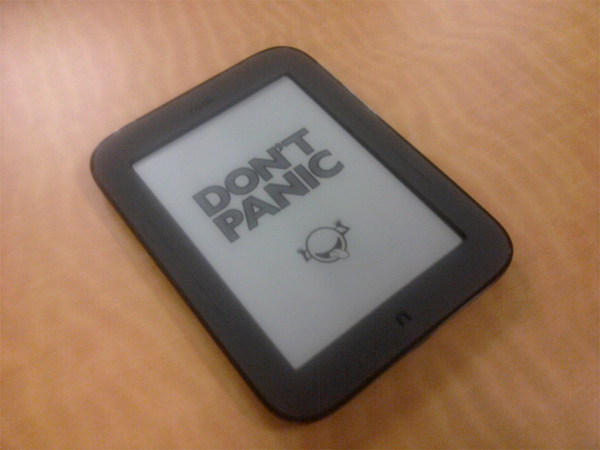
\includegraphics[height=0.25\textheight]{pictures/nook_simple_touch.jpg} \\
                A imagem acima, de Quillaja, encontra-se dispon\'{i}vel em \url{http://en.wikipedia.org/wiki/File:Sony_reader_showing_pride_and_prejudice.jpg} e em dom\'{i}nio p\'{u}blico. & A imagem acima, de Difbobatl, encontra-se dispon\'{i}vel em \url{http://en.wikipedia.org/wiki/File:Kindle4.jpg} e regulada nos termos da licen\c{c}a Creative Commons - Atribui\c{c}\~{a}o - Partilha nos Mesmos Termos 3.0 N\~{a}o Adaptada. & A imagem acima, de Dhbillings, encontra-se dispon\'{i}vel em \url{http://en.wikipedia.org/wiki/File:Nook_Simple_Touch_With_%22Don%27t_Panic!%22.jpg} e regulada nos termos da licen\c{c}a Creative Commons - Atribui\c{c}\~{a}o - Partilha nos Mesmos Termos 3.0 N\~{a}o Adaptada.
            \end{tabular}
        \end{center}
    \end{tiny}
\end{frame}

\begin{frame}
    \frametitle{1999-\dots}
    \begin{description}
        \item[1999] Lan\c{c}ado Open eBook Publication Structure 1.0.
        \item[2002] Lan\c{c}ado Open eBook Publication Structure 2.0.
        \item[2007] Lan\c{c}ado Open Publication Structure 2.0.
        \item[2011] Lan\c{c}ado EPUB 3.0.
    \end{description}
\end{frame}

\begin{frame}[fragile]
    \frametitle{EPUB}
    \begin{lstlisting}
file.epub
    mimetype
    META-INF/
        container.xml
    OEBPS/
        content.opf
        cover.html
        text_of_book.html
    \end{lstlisting}

    Exceto pelo \lstinline!mimetype!, todos os arquivos s\~{a}o XML.
\end{frame}

\begin{frame}
    \frametitle{Algumas conclus\~{o}es pessoais}
    \begin{itemize}
        \item O LaTeX \'{e} uma tecnologia f\'{a}cil de utilizar, est\'{a}vel e madura.
            \pause
        \item O PDF \'{e} uma tecnologia bastante difundida e em sua \'{u}ltima vers\~{a}o possue v\'{a}rios recursos, e.g., anota\c{c}\~{o}es e marca\c{c}\~{o}es.
            \pause

            \'{E} importante destacar que no Linux o \'{u}nico leitor com estes recursos \'{e} o Okular que utilizar arquivo pr\'{o}prio para esta finalidade. O motivo da falta desses recursos decorre da biblioteca utilizada para visualizar os arquivos.
            \pause
        \item Para conte\'{u}do din\^{a}mico n\~{a}o h\'{a} nada melhor do que o HTML.
            \pause
            
            \'{E} bastante irritante ter que duplicar c\'{o}digo para manter compatibilidade entre \textit{engines}. E nada mais frustrante que \textit{engines} inacabadas, e.g., a WebKit n\~{a}o possue suporte ao MathML.
            \pause
        \item O EPUB n\~{a}o \'{e} muito f\'{a}cil e sofre dos mesmos problemas do HTML.
    \end{itemize}
\end{frame}

\begin{frame}
    Obrigado.
\end{frame}
\end{document}
